%\documentclass{article}
%\usepackage{graphicx}
%
%\begin{document}
%	\section{Introduction}
		Industrial robots are reshaping the present and future of most, and very soon all, industrial aspects. They are currently used in a broad spectrum of industries, some of which include car parts assembly as in BMW and Mercedes factories, industrial automation as in Yaskawa factories, metal industries that include welding and machining processes and many others. While there is a controversial part in replacing humans with robots in factories, it, nevertheless, offers more accuracy and higher production rate with more space for development. The growth of the Global Industrial Robotics Market is driven by many factors, of which the need to reduce manufacturing cost in industries is one of the main drivers. Industrial robotics aids companies in reducing the cost due to product failure and product wastage.

\bigskip			
	Some of the pioneering companies in the Industrial robotics market are ABB Ltd., Fanuc Corp., Yaskawa Electric Corp., Apex Automation and Robotics, Mistubishi Electric Corp. and KUKA AG. We had the opportunity to work with the latter, KUKA AG, on the implementation of our project (\emph{ZuKa: Deployment of the industrial KUKA robotic manipulator in CNC machining and visual servoing through Kinect interfacing on ROS}). Over the course of our final year, this project helped increase our knowledge, not only on the main topic, milling and visual servoing, but also on the KUKA platform itself, which is considered an advanced platform widely used in today’s industries. 
\begin{figure}[h]
    \centering
    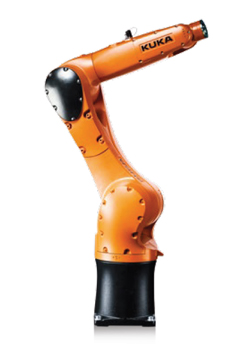
\includegraphics[width=0.7\linewidth]{figures/kuka}
    \caption{KUKA KR6 R900 sixx robotic manipulator}
    \label{fig:kuka}
\end{figure}

	The milling process witnessed vast development since the early milling machines, known as mills, followed by CNC milling machines and all the way to milling robots. The latter, represented in KUKA robots in our project, can be compared to CNC machines in terms of introducing a computer-based control method, however, milling robots offers more advantages than the conventional CNC machines. One of these advantages is flexibility, because as the needs of manufacturing evolve; robots are proving to be nimble adjusters. 
	
\bigskip	
	
	In addition to robots’ ability to perform several tasks; by adding the desired end effector and designing the corresponding programming tool, they offer more variations of one task offered by a conventional machine. To verify this we can compare CNC milling machines and milling robots. CNC machines offer two-dimensional milling operations, moving either horizontally or vertically with fixed workpiece, resulting in a defined scope of products and processes. Milling robots on the other hand, are able to perform milling in up to five axes, providing rotation and movement in multiple directions. This flexibility can further be improved by providing a movable workpiece fixation, increasing the motion axes to nine.
	
	
	Milling robots offer ease of use through programming, flexibility, speed, precision, cost reduction, repeatability and some of these robots even offer different mounting choices, as they could be mounted on ceilings and walls not just floors. All of this contributed to the current status of milling operations; in terms of final finishing, level of details obtained, rate of production and future possibilities for development. 
	
	
	The project is inspired by the aforementioned development in the industrial sector. The scope of the project can be summarized in the following three points; firstly, the commissioning and operation of the KUKA KR6 R900 sixx robotic manipulator, which included the installation of the related software and creating a network that facilitates communications with the robot. In addition to software commissioning, hands-on experience with the KUKA robot language (KRL) platform was achieved through learning the basic and advanced forms of KRL, which later helped in the development of software tools that facilitates the main objective of the project; the milling process. 
	
\smallskip	
	Secondly, the design and manufacturing of a base to support the robot during heavy duty operation, this included performing mathematical calculations based on the robot’s weight and forces to obtain the optimal dimensions and weight for the base, besides performing CAD studies on the manipulator’s body to support the results of the mathematical analysis. 
	
\medskip
	
	Finally, the development of various software tools to achieve the purposes of remotely controlling the robot and milling. These tools include an Inkscape extension for converting 2D G-code to KRL, directly using sketches from Inkscape, an independent toolkit for converting 3 axis G-code to KRL. In addition to Python tools; one Python class for reading and writing system variables, and a Python library for controlling the arm motions from pc. The development also included editing openni\_tracker for publishing uncalibrated person's depth and creating ROS nodes for safety operation distance and visual servoing (hand guiding) for the robot.
	
	Initially, the project scope was limited to the milling process in addition to minor ideas in the smart development of the workspace, however, over the course of the semester we encountered many problems that required extended research in all the previously mentioned aspects, which eventually led to broadening the scope of the project to include these development tools, both relevant and irrelevant to milling. 

\section{Project Contributions}
	The results of the project studies and implementation include, but not limited to; 
\begin{itemize}
	\item The manufacturing of the robot’s base, with mathematically calculated data endorsed by CAD studies, contributing in a stable, secure and robust base that can support the weight of the robot and tolerate the forces resulting from the robot’s motion without major failure or errors.
	\item The attachment and operation of a pneumatic gripper, leading to the development and implementation of software tools for drawing and palletizing.
	\item The development of different software tools to obtain the appropriate KRL codes used in the milling process.
	\item The development of a safety system in the robot’s workspace, similar to KUKA AG’s own Collision detection, which stops thee robot from moving when it hits a solid surface. However, being more efficient and safe, in terms that it does not require actual contact or collision but significantly reduced the operation speed of the robot when someone enters a defined perimeter of the robot’s workspace. This is achieved using a Microsoft Kinect device for obtaining visual input of the workspace.
\end{itemize}

	The results of the work exceeded both the preset expectations and goals for the project, resulting in a wide variety of applications and an extension in our own knowledge base, which is the most important achievement. 

	\section{References}
	\begin{enumerate}
		\item http://www.mmsonline.com/articles/a-new-milling-101-what-milling-is-then-and-now-plus-a-glossary-of-milling-terms
		\item http://www.sickinsight-online.com/safety-and-more-sick-provides-protection-and-navigation-data-for-kukas-kmr-iiwa/ 
		\item http://medicaldesign.com/contract-manufacturing/modern-cnc-machining-prescription-product-development 
		\item http://articles.sae.org/11272/ 
		\item https://en.wikipedia.org/wiki/Multiaxis\_machining 
		\item https://en.wikipedia.org/wiki/Milling\_(machining) 	
	\end{enumerate}
	

%\end{document}